%% V1.0
%% by Shingo Mori, spawn.s.mori@gmail.com

\documentclass[10pt,journal,compsoc]{IEEEtran}

\usepackage[pdftex]{graphicx}    
\usepackage{cite}
\usepackage{subfig}
\hyphenation{op-tical net-works semi-conduc-tor}


\begin{document}

\title{Where Am I? Writeup}

\author{Shingo Mori}

\markboth{Localization project, Robotics Nanodegree Program, Udacity}%
{}
\IEEEtitleabstractindextext{%

\begin{abstract}
A ROS package is created and mobile robots performing 2D navigation in a gazebo environment is implemented. ROS packages included in Navigation Stack are used and their parameters are tuned to improve the localization results. Two models, Benchmark Model and Personal Model, are created. Parameters are configured for each model, and both robots are able to reach the goal with reasonable localization accuracy.
\end{abstract}

\begin{IEEEkeywords}
Udacity, ROS, SLAM, Navigation Stack, AMCL.
\end{IEEEkeywords}}

\maketitle
\IEEEdisplaynontitleabstractindextext
\IEEEpeerreviewmaketitle
\section{Introduction}
\label{sec:introduction}

\IEEEPARstart{L}{ocalization} is the most basic perceptual problem in robotics. Almost all the mobile robot require knowledge of its location. Since the pose of a robot usually can not be measured directly, it must be inferred from input data. To deal with various uncertainties that come from the real world, an probabilistic approach \cite{Thrun:2005:PR:1121596} is widely applied. 

There are three types of localization problems: Position tracking, global localization, and kidnapped robot problem. Position tracking, also called as local problem, is the easiest of all. The initial pose of a robot is known, so the localization is done by filtering out the measurement noise as the robot moves around. Methods for position tracking often assume pose uncertainty is small. In global localization, the initial robot pose is unknown. The pose uncertainty is not bounded to local regions near the robot, which makes the problem more difficult than position tracking. Kidnapped robot problem, a variant of global localization, is even more difficult. A robot gets teleported to another location during the operation. The robot has to properly abandon the wrong belief of its pose and recover from the failure.

Another thing that has critical impact on localization problem is the environment. An environment where the robot is the only object that moves is called a static environment. On the contrary, an environment containing other objects that change their pose over time, it is called a dynamic environment. Localization in a dynamic environments is obviously more difficult than localization in a static one.

In this project, a ROS package is created to solve global localization problem in a static environment. A  mobile robot spawns in a gazebo environment as shown in Fig. \ref{fig:environment} and attempts to move to its final pose. The goal of this project is to utilize ROS packages to accurately localize the robot and successfully navigate it to the goal position.

\begin{figure}[thpb]
      \centering
      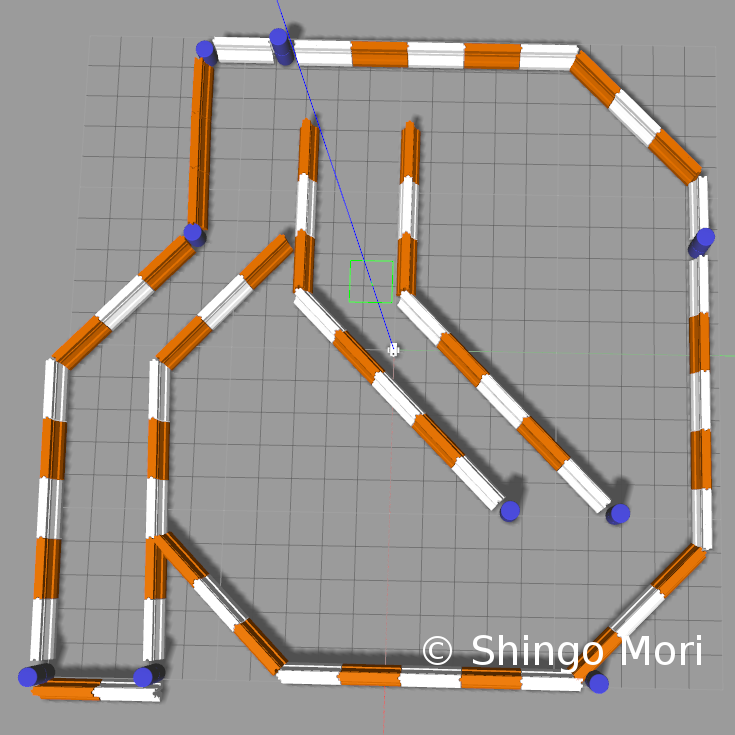
\includegraphics[width=\linewidth]{gazebo-map}
      \caption{2D navigation environment.}
      \label{fig:environment}
\end{figure}

\section{Background}
There are several approaches to perform localization. Two major methods, the Kalman Filter and the Particle Filter, are covered in the classroom \cite{Udacity:nd209}. Each method is a derivative of the Bayes Filter, an algorithm that recursively updates its belief distribution using incoming sensor and control data.

\subsection{Kalman Filters}
Implementations of the Kalman Filter represent their beliefs by Gaussian distribution. Hence the algorithm assumes the unimodal distribution around the true pose of the robot. Because of its computational efficiency, Kalman Filters are applied to many tracking problems in robotics, where the posterior is often focused around the true pose with a limited amount of uncertainty.

\subsection{Particle Filters}
Particle Filters are implementations of the Non-parametric Filter, where the posterior belief is represented by a finite number of hypothetical values. In Particle Filters, those values are represented by random samples of robot state. They do not assume mathematical form of posterior. Hence their state space is multimodal and distinct.

\subsection{Comparison / Contrast}
Particle Filters have various advantages over Kalman Filters.
First, Particle Filters solve global localization problem better than Kalman Filters, and some implementations can even solve kidnapped robot problems. This is because of the multi-modal and distinct characteristics of Particle Filters. Second, Particle Filters can represent measurement noises as non-Gaussian distribution. This is useful when measurement noises often do not follow the Gaussian distribution, which is often the case in the real world. Third, the computational usage of Particle Filters can be controlled by configuring the number of particles. This is critical in robotics where computational resource is often limited. For the above reasons, an implementation of the Particle Filter is used in this project to solve global localization problem.

\section{Simulations}
A ROS package is created and configured to perform 2D global localization and navigation in a Gazebo environment. Two different robot models, a benchmark model and a personal model are specified in the Unified Robot Description Format (URDF). ROS packages provided in Navigation Stack \cite{ROS:navigation} are used and their parameters are configured. RViz is used to visualize ROS topics.

All the simulation is conducted using ROS Kinetic on Ubuntu 16.04 LTS system with a Core i7-7700 CPU, two 8 GB DDR4 memories, and a NVIDIA GeForce GTX1080Ti GPU. 

\begin{figure}[thpb]
      \centering
      \subfloat[Start pose. The belief is initially spread around the robot.]{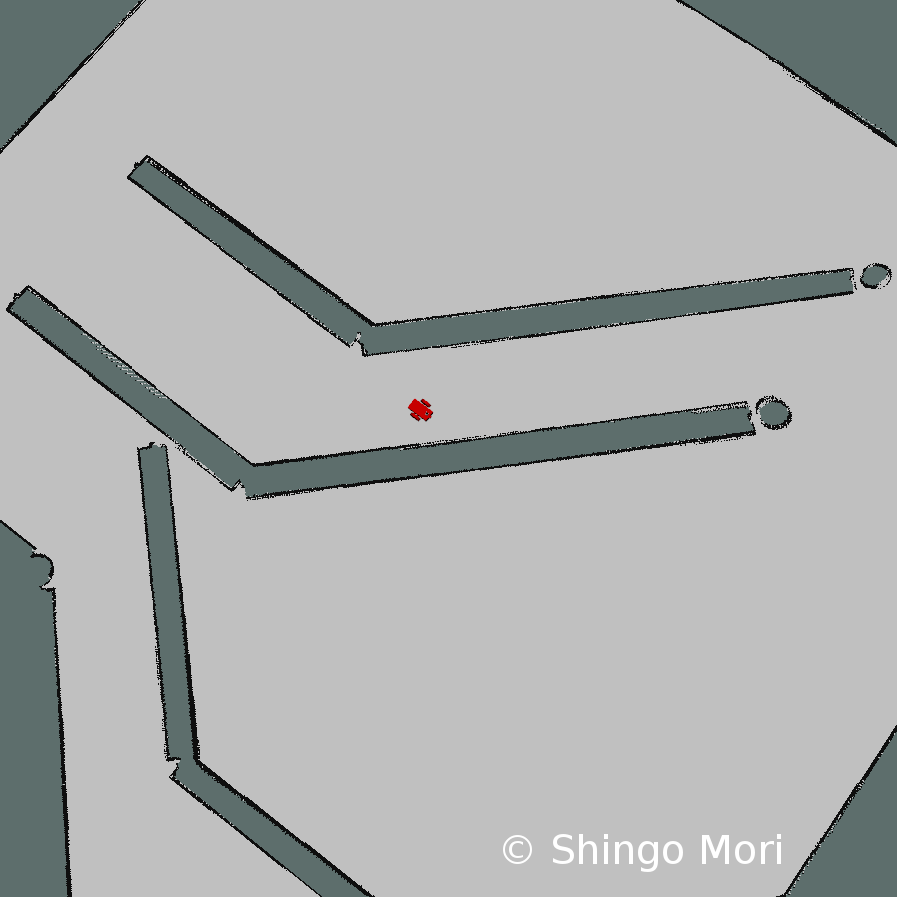
\includegraphics[width=0.45\linewidth]{start-pose}\label{fig:initial-pose}}
      \hfill
      \subfloat[Goal pose. This is specified in the provided .cpp file by Udacity.]{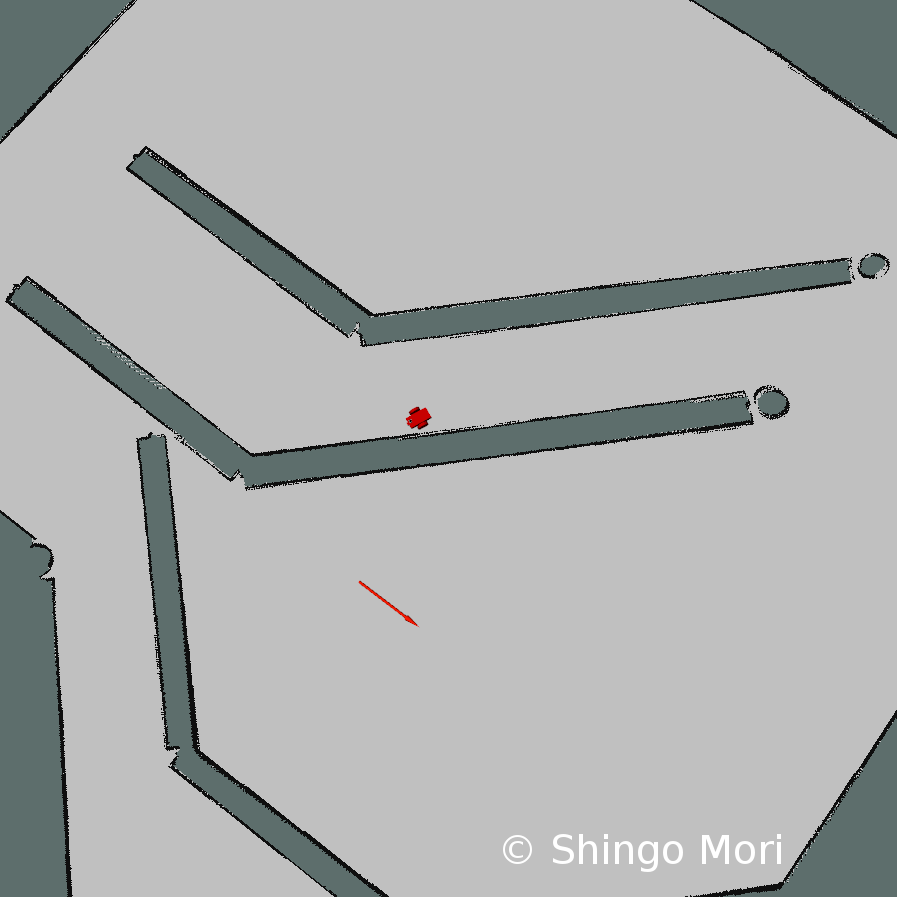
\includegraphics[width=0.45\linewidth]{goal-pose}\label{fig:final-pose}}
      \caption{Start and goal poses.}
\end{figure}

\subsection{Achievements}
2D global localization and navigation are achieved on both the benchmark model and the personal model. Fig. \ref{fig:initial-pose} shows the initial robot pose and Fig. \ref{fig:final-pose} shows the goal pose of the robot. Green arrows represent particles created by the amcl package.

\begin{figure}[thpb]
\centering
  \subfloat[Benchmark Model] {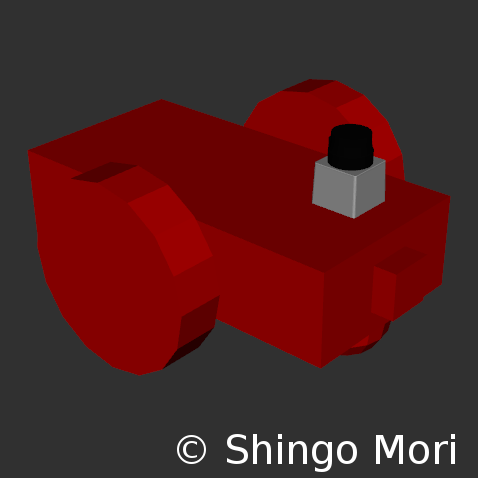
\includegraphics[width=0.45\linewidth]{bench-model}\label{fig:bench-model}}
  \hfill
  \subfloat[Personal Model]{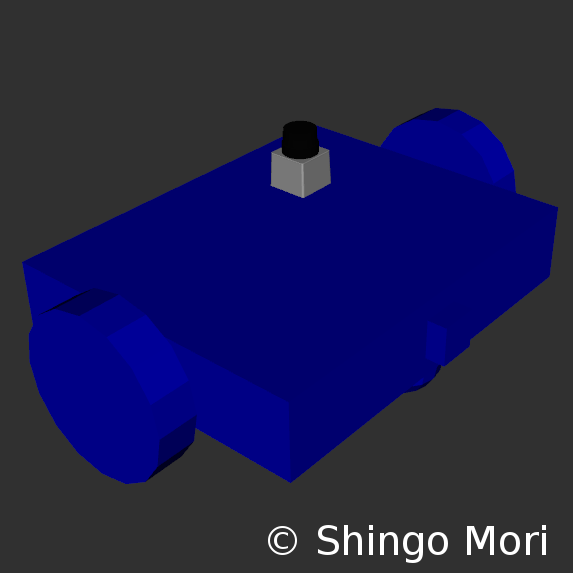
\includegraphics[width=0.45\linewidth]{personal-model}\label{fig:personal-model}}
  \caption{Robot models.}
\end{figure}

% Robot Models
\subsection{Benchmark Model}
\subsubsection{Model design}
The benchmark model has a rectangular chassis (size=0.4m, 0.2m, 0.1m) with two spherical caster on the bottom and two wheels on the side. A camera and a laser range finder are attached to sense the environment. Inertial and collision parameters are specified to each links. An image of the model is shown in Fig. \ref{fig:bench-model}.

\subsubsection{Packages Used}
A ROS package is created and other packages such as amcl \cite{ROS:amcl}, base\_local\_planner \cite{ROS:base-local-planner}, and costmap\_2d \cite{ROS:costmap-2d} included in the Navigation Stack are utilized. The package uses the global map created and provided by Udacity.

The created package subscribes to sensor messages and publishes velocity commands.

\subsubsection{Parameters}
Parameters included in the Navigation Stack are configured. Only the parameters that have impact on the performances of the localization and the navigation are described in this section.

Parameters for the amcl package is shown in TABLE \ref{tab:bench-amcl}. min\_particles, max\_particles and transform\_tolerance are configured based on the system resource. laser\_min\_range and laser\_max\_range are set according to the specification of the sensor. Because odom\_alpha{1-4} determine the uncertainty of the motion model, they have major impact on the localization accuracy. Since the controller noise of the robot is small, setting them to smaller values leads to a better result.

\begin{table}[h]
\caption{Benchmark Model: amcl parameters}
\label{tab:bench-amcl}
\begin{center}
\begin{tabular}{|c|c|c|}
\hline
name & value & default \\
\hline
\hline
min\_particles & 100 & 100 \\
\hline
max\_particles & 1000 & 5000 \\
\hline
transform\_tolerance & 0.5 & 0.1\\
\hline
laser\_min\_range & 0.1 & -1.0\\
\hline
laser\_max\_range & 30.0 & -1.0\\
\hline
odom\_alpha\_1 & 0.001 & 0.2\\
\hline
odom\_alpha\_2 & 0.001 & 0.2\\
\hline
odom\_alpha\_3 & 0.001 & 0.2\\
\hline
odom\_alpha\_4 & 0.001 & 0.2\\
\hline
\end{tabular}
\end{center}
\end{table}

Parameters for the base\_local\_planner package is shown in TABLE \ref{tab:bench-base-local-planner}. holonomic\_robot is set to false because a differential robot is non-holonomic in a 2D environment. sim\_time and pdist\_scale are increased to prevent poor local path-planning which results in the robot running into a infinite loop movement.

\begin{table}[h]
\caption{Benchmark Model: base\_local\_planner parameters}
\label{tab:bench-base-local-planner}
\begin{center}
\begin{tabular}{|c|c|c|}
\hline
name & value & default \\
\hline
\hline
holonomic\_robot & false & true \\
\hline
xy\_goal\_tolerance & 0.4 & 0.10 \\
\hline
yaw\_goal\_tolerance & 0.2 & 0.05 \\
\hline
sim\_time & 5.0 & 1.0\\
\hline
pdist\_scale & 0.7 & 0.6\\
\hline
\end{tabular}
\end{center}
\end{table}

Parameters for the costmap\_2d package is shown in TABLE \ref{tab:bench-costmap-2d}. There are two types of costmap, the global costmap and the local costmap. Common parameters are applied to both costmaps, while other parameters are configured for each. transform\_toloerance, update\_frequency and publish\_frequency are configured based on the system resource. robot\_radius and inflation\_radius are decreased to give more space for the robot to move around. obstacle\_range and raytrace\_range are increased to improve the efficiency of creating the local and global costmaps.

Width and height for the global costmap are set to 40 to cover the entire environment. static\_map is set to true since the global costmap uses the provided map to create its costmap.

Setting width and height to 20 for local costmap is sufficient for the local path-planning. static\_map is set to false to create and maintain its own map.

\begin{table}[h]
\caption{Benchmark Model: costmap\_2d parameters}
\label{tab:bench-costmap-2d}
\begin{center}
\begin{tabular}{|c|c|c|}
\hline
name & value & default \\
\hline
\hline
\multicolumn{3}{|c|}{common} \\
\hline
transform\_tolerance & 0.5 & 0.2 \\
\hline
robot\_radius & 0.4 & 0.46\\
\hline
inflation\_radius & 0.4 & 0.55\\
\hline
obstacle\_range & 0.3 & 0.25\\
\hline
raytrace\_range & 0.4 & 0.3\\
\hline
\multicolumn{3}{|c|}{global costmap} \\
\hline
update\_frequency & 10.0 & 5.0 \\
\hline
publish\_frequency & 5.0 & 5.0 \\
\hline
width & 40 & 10 \\
\hline
height & 40 & 10 \\
\hline
static\_map & true & true \\
\hline
rolling\_window & false & false \\
\hline
\multicolumn{3}{|c|}{local costmap} \\
\hline
update\_frequency & 10.0 & 5.0 \\
\hline
publish\_frequency & 5.0 & 5.0 \\
\hline
width & 20 & 10 \\
\hline
height & 20 & 10 \\
\hline
static\_map & false & true \\
\hline
rolling\_window & true & false \\
\hline
\end{tabular}
\end{center}
\end{table}

\subsection{Personal Model}
\subsubsection{Model design}
Basic structure of the personal model is similar to the benchmark model, but with larger chassis (size=0.4m, 0.5m, 0.1m) and different placement of the laser range finder. An image of the model is shown in Fig. \ref{fig:personal-model}.

\subsubsection{Packages Used}
Packages used for the personal models are the same as those used for the benchmark model.

\subsubsection{Parameters}
Most parameters for the personal model are the same as those for the benchmark model. Only the parameters configured specifically for the personal model are described in this section.

Parameters for the costmap\_2d package is shown in TABLE \ref{tab:personal-costmap-2d}. robot\_radius is set according to the size of the robot. inflation\_radius is set to maintain the same obstacle-free space as the one for the benchmark model.

\begin{table}[h]
\caption{Personal Model: costmap\_2d parameters}
\label{tab:personal-costmap-2d}
\begin{center}
\begin{tabular}{|c|c|c|}
\hline
name & value & default \\
\hline
\hline
\multicolumn{3}{|c|}{common} \\
\hline
robot\_radius & 0.5 & 0.46\\
\hline
inflation\_radius & 0.3 & 0.55\\
\hline
\end{tabular}
\end{center}
\end{table}

\section{Results}
\label{sec:results}
Both the benchmark model and the personal model reaches the goal with sufficient localization accuracy. Although the robot drifts away from the global path when it starts its first movement (Fig. \ref{fig:result-drift-away}), it comes back to the correct path after moving around a several seconds (Fig. \ref{fig:result-following-path}). After retuning to its correct path, the robot moves smoothly to the goal position without being stuck (Fig. \ref{fig:result-corner} and Fig. \ref{fig:result-goal}). Duration of the time for the robot to reach the goal is around around 90 seconds with the benchmark model, and around 100 seconds with the personal model.

\begin{figure}[thpb]
      \centering
      \subfloat[Initially drifting away from its global path-plan.]{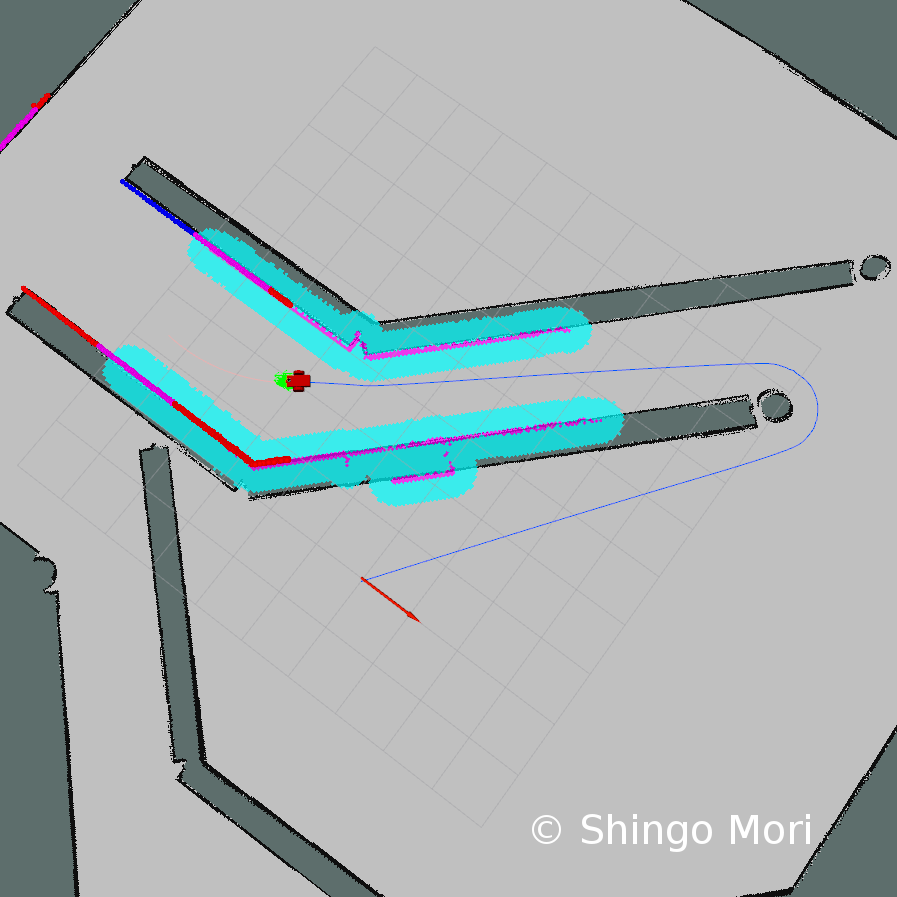
\includegraphics[width=0.45\linewidth]{result-drift-away}\label{fig:result-drift-away}}
      \hfill
      \subfloat[Returning to and start following the global path-plan.]{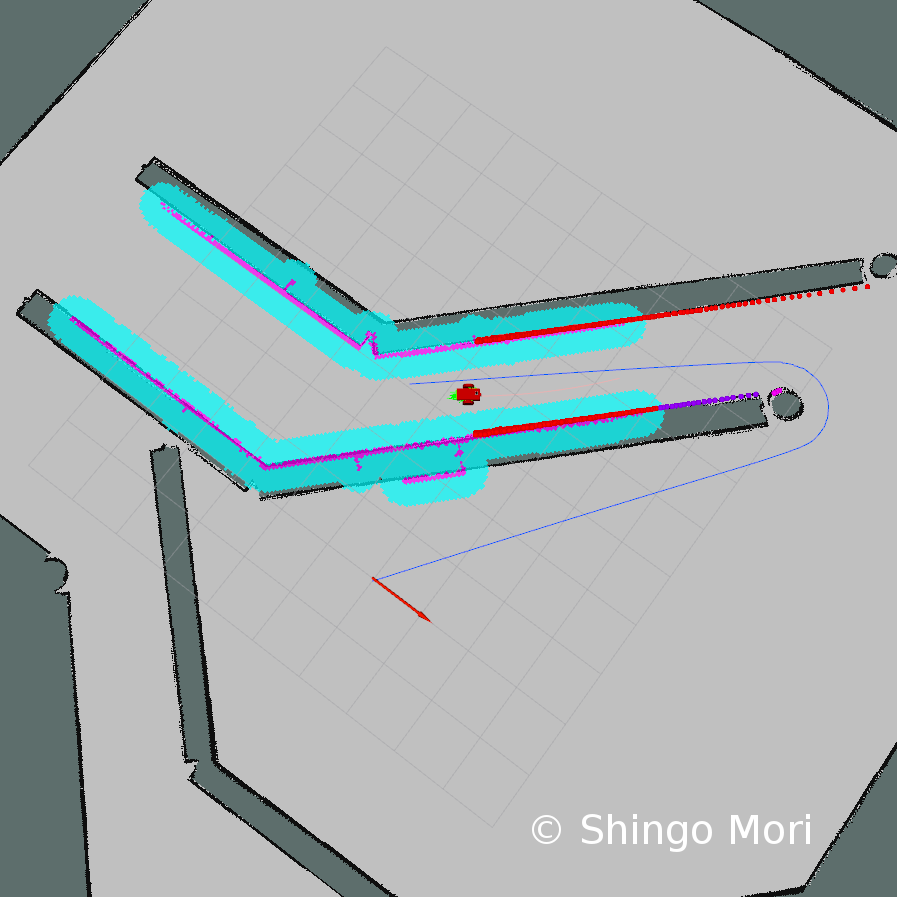
\includegraphics[width=0.45\linewidth]{result-following-path}\label{fig:result-following-path}}
      \vfill
      \subfloat[Passing the corner without being stuck.]{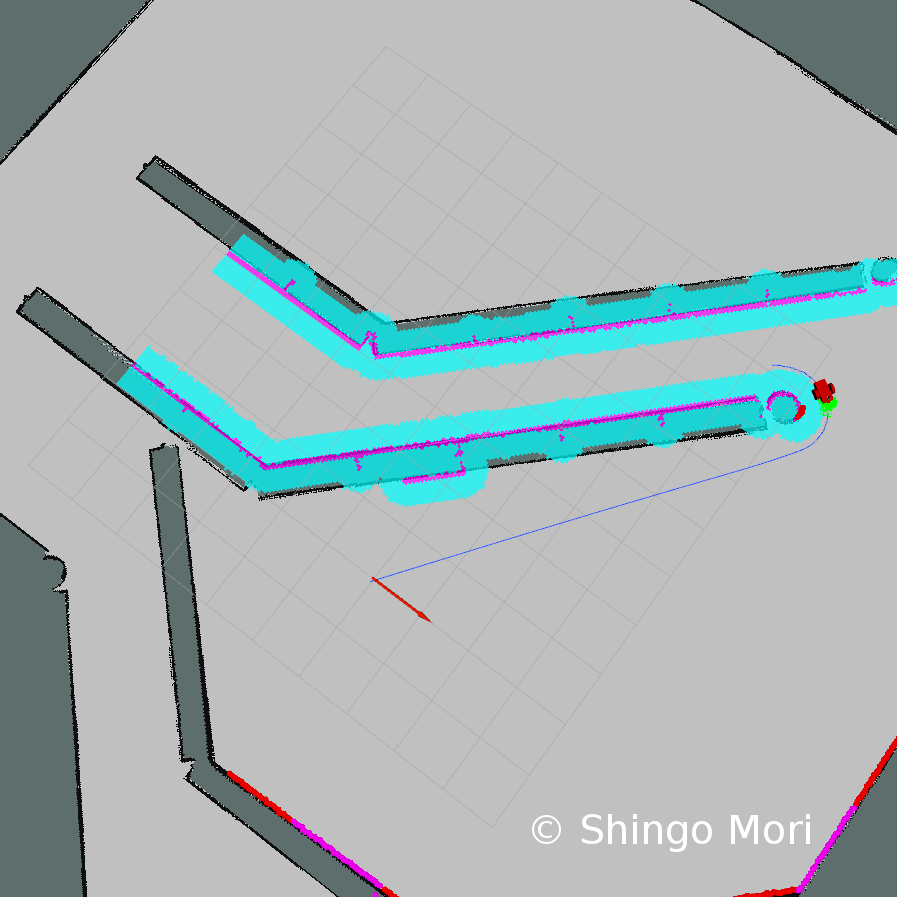
\includegraphics[width=0.45\linewidth]{result-corner}\label{fig:result-corner}}
      \hfill
      \subfloat[Reaching the goal pose.]{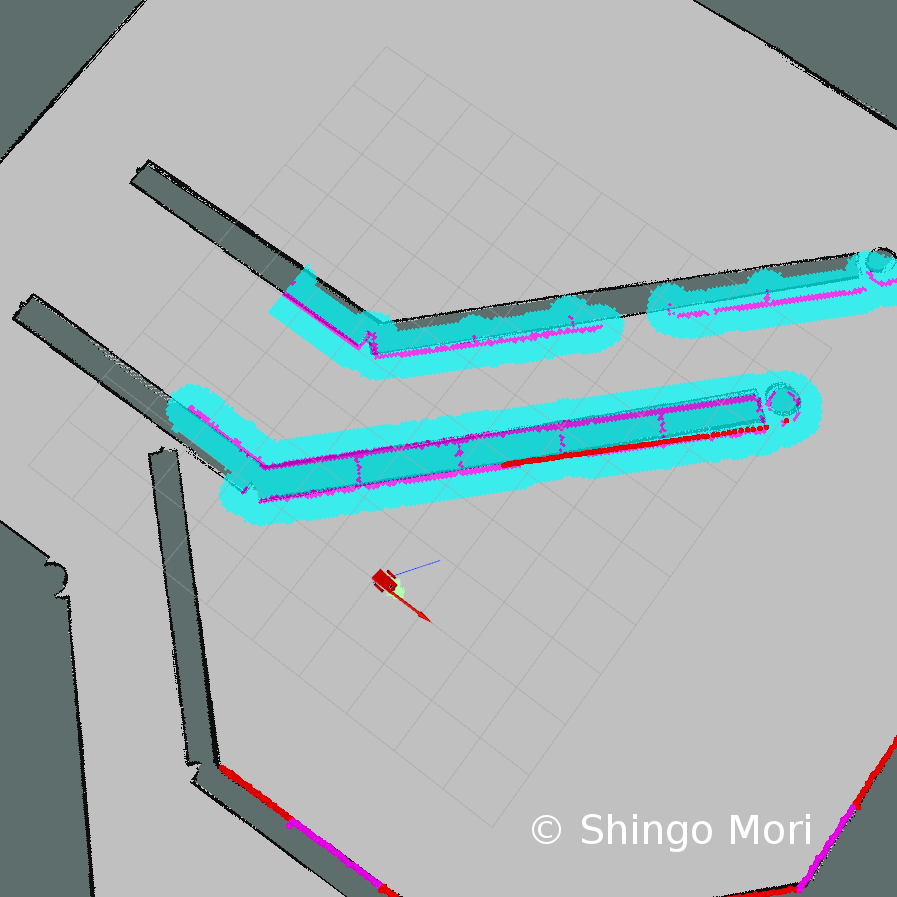
\includegraphics[width=0.45\linewidth]{result-goal}\label{fig:result-goal}}
      \caption{Resulting movements.}
\end{figure}

\subsection{Localization Results}
\begin{figure}[thpb]
      \centering
      \subfloat[Benchmark Model]{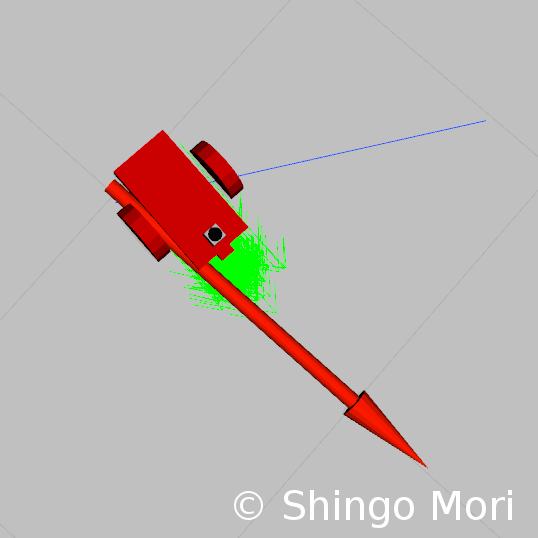
\includegraphics[width=0.45\linewidth]{bench-localization-result}\label{fig:bench-localization-result}}
      \hfill
      \subfloat[Personal Model]{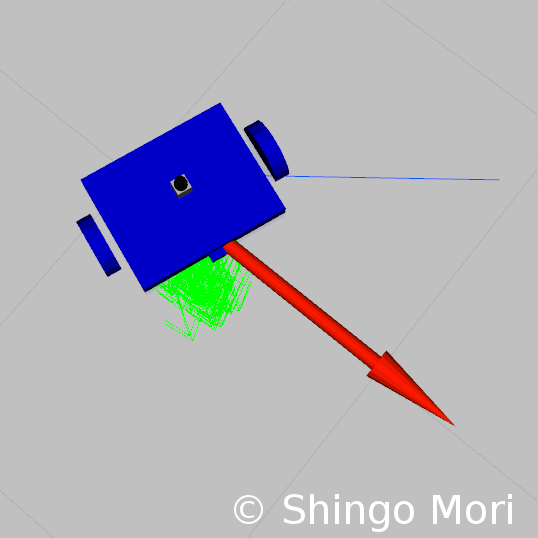
\includegraphics[width=0.45\linewidth]{personal-localization-result}\label{fig:personal-localization-result}}
      \caption{Localization Results.}
\end{figure}

\subsubsection{Benchmark Model}
As shown in Fig. \ref{fig:bench-localization-result}, the benchmark model is localized accurately at the goal position. It took around 15 seconds for the particle filter to converge.

\subsubsection{Personal Model}
As Fig. \ref{fig:personal-localization-result} shows, the localization result of personal model is quite similar to the one from the benchmark model. It took around 15 seconds for the particle filter to converge.

\subsection{Technical Comparison}
\label{sec:technical_comparison}
The personal model has wider chassis than the benchmark model. This caused  it harder for the personal model to curve. However, after configuring the inflation\_radius, and the personal model is able to move around as freely as the benchmark model. Although the layout and the sensor position of the personal model is changed from the benchmark model, the noise parameters of the sensor model and the motion model remains the same. Hence, the localization accuracy stays almost the same despite the changes made on the layout.

\section{Discussion}
The performance of the benchmark model and the personal model are almost the same as mentioned in the section \ref{sec:technical_comparison}. This is because changing the layout did not affect the controller noise and the measurement noise of the robot.

Dealing with the parameters for the base\_local\_planner was the hardest. As described in the section \ref{sec:results}, the robot initially drifts away from the global path. Since the weight of local path-planning is high, the robot seems to 'prefer' the local path over the global path if there is a conflict between the two. This causes the robot drifting away. However, simply increasing the weight of the global path-planning is not a straight forward solution; It reduces the flexibility of the overall path-planning and results in getting easily stuck in walls and corners. pdist\_scale and sim\_time must be carefully configured to get a good balance.

Particle filters converges quite easily by setting the small values to odom\_alpha{1-4}. However, this is because the odometry noise and the measurement noise are small in this project. Noise parameters should be configured more carefully if the environment is more dynamic or noises are more significant.

Although the algorithm implemented in the amcl package is capable of solving the kidnapped problem, this feature is disabled by default. recovery\_alpha\_slow and recovery\_alpha\_fast must be set and configured properly for the algorithm to solve the problem.

This package can be used in an industry domain since the localization accuracy and the frequency (over 5Hz) is sufficiently high. However, some parameters should be configured in accordance to the system requirement.

\section{Conclusion / Future work}
Two models, Benchmark Model and Personal Model, performing 2D global localization and navigation are implemented in a ROS package. Both models generally follow their global path and reach the goal without being stuck in objects like walls and corners. The localization accuracy is high while the processing time remains reasonable. Adaptive characteristic of the amcl algorithm enables users to deploy the package on embedded hardwares just by configuring a few parameters.

For future work, the package is deployed on an actual device and tested outside of the simulated environment. Some parameters should be configured to meet the system requirement and deal with the complexity of the real world.

\bibliography{bib}
\bibliographystyle{ieeetr}

\end{document}